\documentclass[10pt,executivepaper]{article}
\usepackage[utf8]{inputenc}
\usepackage[spanish]{babel}
\usepackage{amsmath}
\usepackage{amsfonts}
\usepackage{amssymb}
\usepackage{graphics}
\usepackage{graphicx}
\usepackage[left=2cm,right=2cm,top=2cm,bottom=2cm]{geometry}
\usepackage{imakeidx}
\makeindex[columns=3, title=Alphabetical Index, intoc]
\usepackage{listings}
\usepackage{xcolor}
\usepackage{multicol}
\usepackage{changepage}
\usepackage{float}
\usepackage{cite}
\usepackage{url}
\usepackage{pdflscape}

\definecolor{codegreen}{rgb}{0,0.6,0}
\definecolor{codegray}{rgb}{0.5,0.5,0.5}
\definecolor{codepurple}{rgb}{0.58,0,0.82}
\definecolor{backcolour}{rgb}{0.95,0.95,0.92}

\lstdefinestyle{mystyle}{
    backgroundcolor=\color{backcolour},
    commentstyle=\color{codegreen},
    keywordstyle=\color{magenta},
    numberstyle=\tiny\color{codegray},
    stringstyle=\color{codepurple},
    basicstyle=\ttfamily\footnotesize,
    breakatwhitespace=false,
    breaklines=true,
    captionpos=b,
    keepspaces=true,
    numbers=left,
    numbersep=5pt,
    showspaces=false,
    showstringspaces=false,
    showtabs=false,
    tabsize=3
}

\def\fillandplacepagenumber{%
 \par\pagestyle{empty}%
 \vbox to 0pt{\vss}\vfill
 \vbox to 0pt{\baselineskip0pt
   \hbox to\linewidth{\hss}%
   \baselineskip\footskip
   \hbox to\linewidth{%
     \hfil\thepage\hfil}\vss}}


\lstset{style=mystyle}

\title{Actividad: Chat multicast}

\author{Instituto Politécnico Nacional\\Escuela Superior de Computo\\Desarrollo de Sistemas Distribuidos\\Adrian González Pardo\\4CV1\\21/01}
\date{\today}
\newcommand\tab[1][1cm]{\hspace*{#1}}

\begin{document}
% Portada
%encabezado
\begin{minipage}{0.4\textwidth}
	\begin{flushleft}
		
\includegraphics[scale = 0.05]{logoescom.png}
	\end{flushleft}
\end{minipage}
\begin{minipage}{0.51\textwidth}
	\begin{flushright}
		
\includegraphics[scale = 0.055]{logoipn.png}
	\end{flushright}
\end{minipage}
\begin{center}
	\par\vspace{0.5cm}{
	\huge\textbf{Instituto Politécnico Nacional \\*[0.20cm] Escuela Superior de Cómputo}}
\par\vspace{1cm}{
	\large\textbf{Desarrollo de Sistemas Distribuidos\\Actividad: Multiplicación de matrices utilizando objetos distribuidos\\Curso impartido por el profesor: Pineda Guerrero Carlos\\Grupo: 4CV1\\21/01\\Alumno: Adrian González Pardo\\}
}
\par\vspace{1cm}{
	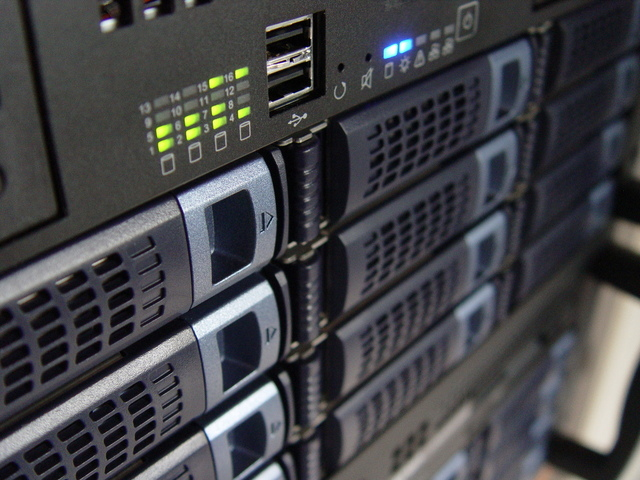
\includegraphics[scale=0.5]{servers.jpg}
}
\par\vspace{2cm}{
	Ultima fecha modificado: \today
}
\end{center}

% Indice
\clearpage
\section{Desarrollo}
Para esta practica es necesario conocer las ip's de nuestras maquinas virtuales las cuales actuaran como nuestro cliente y nuestros servidores de Java RMI, por ello a continuación se mostrara el código fuente y el como se realizo la tarea de enviar los archivos.
\section{Código fuente:}
\begin{center}
  \lstinputlisting[language=Java]{../InterfaceRMI.java}
  \lstinputlisting[language=Java]{../ClaseRMI.java}
  \lstinputlisting[language=Java]{../ServidorRMI.java}
  \lstinputlisting[language=Java]{../ClienteRMI.java}
  \lstinputlisting[language=Bash]{../Makefile}
\end{center}
\section{Ejecución en red}
\textbf{Para la ejecución en red es necesario hacer uso de distintas VM's las cuales ejecutaran en distintas Maquinas Virtuales, el cual se presenta con hostname:ip}\\

\begin{itemize}
  \item ubuntu-azure:52.183.250.226
  \item ubuntu-azure1:52.185.206.51
  \item ubuntu-azure2:52.171.214.166
  \item ubuntu-azure3:13.84.203.145
\end{itemize}
Para comunicarse rápidamente con los equipos se realizo el siguiente script el cual se comunica inicialmente con el e instalar rapidamente los archivos se escribio el siguiente script y en la interfaz de red de la VM aun sea el caso o no de que cada VM este dentro del entorno de trabajo o no es bueno que inicialmente en la configuración de red le configuremos la aceptación del puerto 1099 vía tcp o en cualquier caso cualquiera para que este no sea el problema habilitar tanto el puerto TCP como el UDP para la aplicación.
\begin{center}
  \lstinputlisting[language=Bash]{../script.sh}
\end{center}
Finalmente se escribio un script para enviar los archivos fuente para su ejecución
\begin{center}
  \lstinputlisting[language=Bash]{../scriptScp.sh}
\end{center}
\section{Capturas y descripción del programa}
\begin{center}
  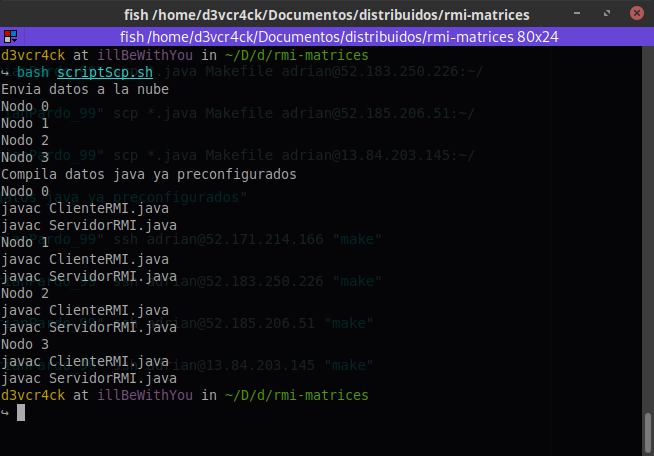
\includegraphics[scale=0.5]{img/scripting-scp.png}
  \\\textit{Figura 1: Ejecución del script para crear enviar los datos a las maquinas virtuales}
  \\
  \begin{landscape}
    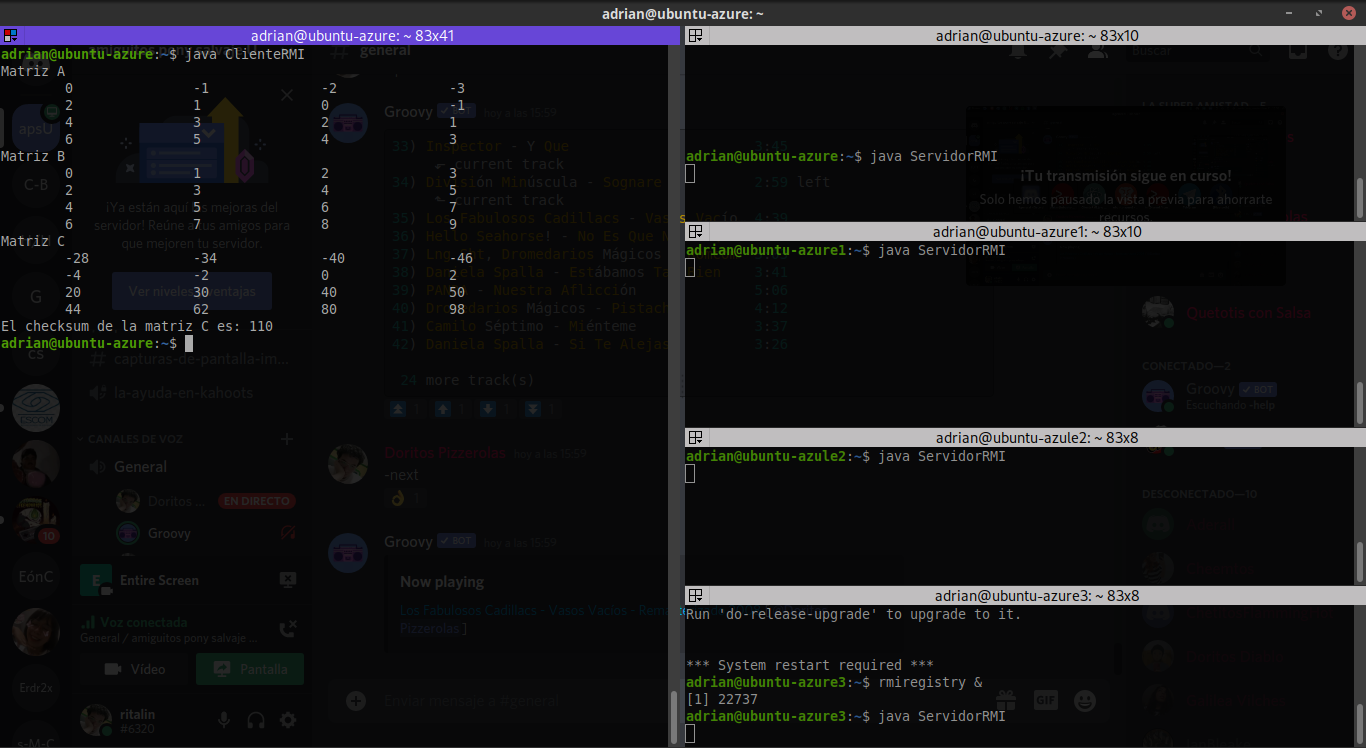
\includegraphics[scale=0.45]{img/ejecucion-N4.png}
    \\\textit{Figura 2: Ejecución en los cuatro nodos con N=4}
    \fillandplacepagenumber
    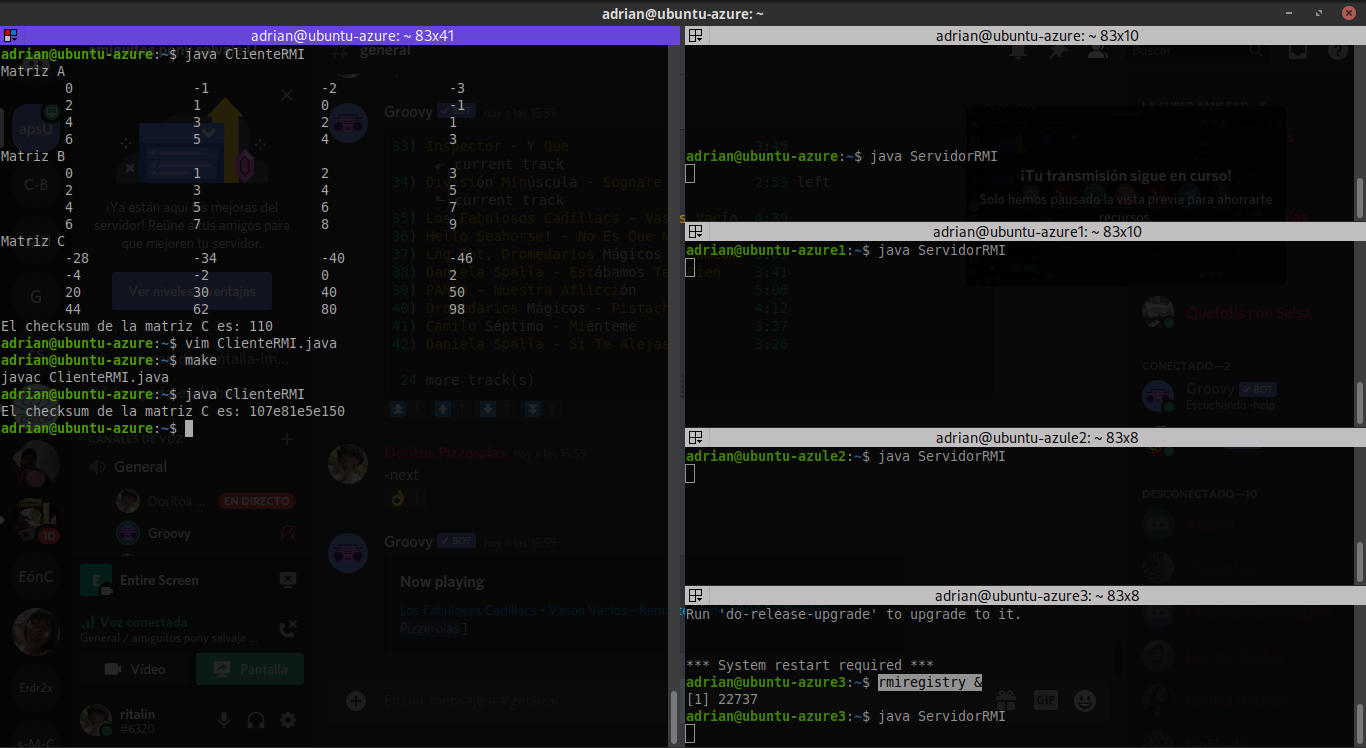
\includegraphics[scale=0.45]{img/ejecucion-N500}
    \\\textit{Figura 3: Ejecución en los cuatro nodos con N=500}
    \fillandplacepagenumber
  \end{landscape}

\end{center}

\section{Conclusiones}
El implementar RMI en esta practica nos permite darnos cuenta de lo sencillo que es implementar el calculo de la multiplicación de matrices que se realizo vía hilos y sockets, que fue más sencillo de implementar con respecto al otro al menos en líneas de código.

\end{document}
